\chapter{Esperimenti}
\section*{Setup testing}
Come anticipato precedentemente, il modello scelto ha un'architettura simile a quella di LeNet-5. Trattandosi di un task di classificazione vicino a quello del riconoscimento di cifre scritte a mano, la scelta di un'architettura ispirata a LeNet-5 è stata naturale, essendo consolidata per questo tipo di problemi.
Sono state comunque effettuate delle modifiche rispetto alla classica architettura sopra citata, sia per adattarla alle features del nostro task di classificazione (che prevedono un paio di input in più), sia per poter ottenere risultati migliori in fase di training (aggiungendo un paio di layer di dropout).
\\
Per poter ottenere la miglior combinazioni di iperparametri, sono stati effettuati diversi esperimenti, variando \emph{learning rate}, \emph{batch size}, \emph{dropout rate}, \emph{momentum} e \emph{numero di epoche}.
Per ognuna delle varianti negli iperparametri nella fase di training, viene generato un log TensorBoard che contiene le coppe di \emph{Loss} e \emph{Accuracy} in entrambi i dataset di training e validation. Inoltre, vengono salvati i pesi al termine delle epoche, utile per poterli ricaricare successivamente.
Di seguito vengono evidenziati gli esperimenti effettuati.

\section{Exps 1}
Il primo esperimento prevede l'iterazione di una griglia di parametri presenti all'interno di un file di configurazione. In particolare, la griglia prevede tutte le triple dei seguenti parametri nei corrispettivi range:
\begin{itemize}
    \item \textbf{Learning rate}: \{0.01, 0.001, 0.005, 0.0001, 0.0005\}
    \item \textbf{Dropout rate}: \{0.2, 0.3, 0.4, 0.5\}
    \item \textbf{Momentum}: \{0, 0.5, 0.9\}
\end{itemize}

Essendo un modello piuttosto piccolo, è stato ritenuto opportuno impostare una batch size di \textbf{2560}, garantendo un calcolo del gradiente più preciso comparato a una batch size piccola. Per semplicità, il numero di epoche è fissato a 50.

Questo approccio di \emph{grid search}, per quanto semplice, potrebbe già restituire dei risultati approssimativi sui range più opportuni per risolvere il problema, rendendo possibile ulteriori esperimenti nei range vicini alla tripla migliore. 

\begin{figure}[htbp]
    \centering
    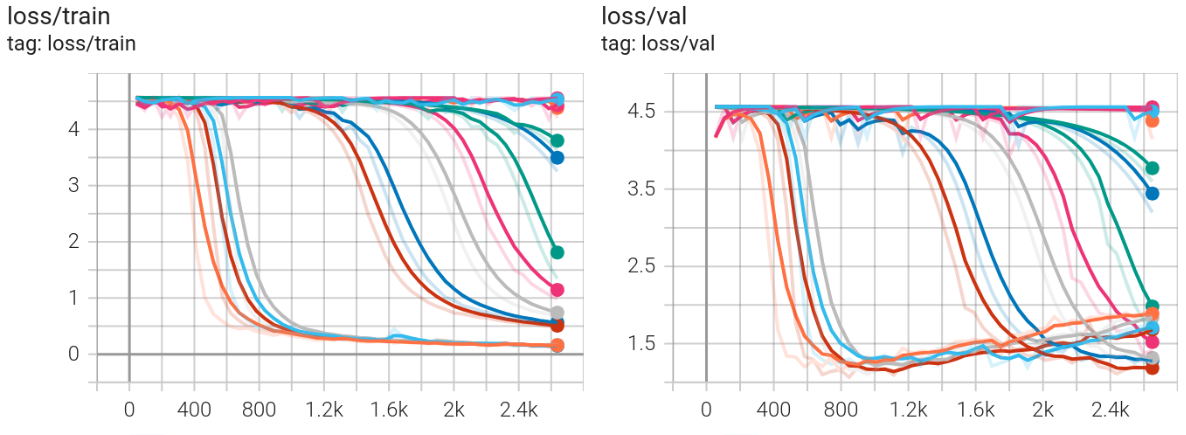
\includegraphics[width=0.8\textwidth]{images/exps1_loss.png}
    \caption{Loss Exps 1}
    \label{fig:exps1_loss}
\end{figure}

Durante la fase di training si è notato come i tempi di training siano dilatati, rendendo questo approccio inefficiente. Inoltre, a colpo d'occhio, durante l'iterazione dei vari iperparametri, si è notato come le prestazioni del modello fossero parecchio scadenti. Qualche training terminava in overfitting evidente, mentre altri sembravano non convergere entro le 50 epoche.

Per queste ragioni, senza ultimare il training con tutte le permutazioni, si è preferito procedere per via iterativa, come approfondito nella sezione successiva.

\section{Exps 2}

La soluzione più efficiente per ottimizzare il flusso precedentemente configurato si è rilevato essere un processo iterativo con l'intervento umano che regola gli iperparametri più opportuni man mano che gli esperimenti avvengono.

\begin{figure}[htbp]
    \centering
    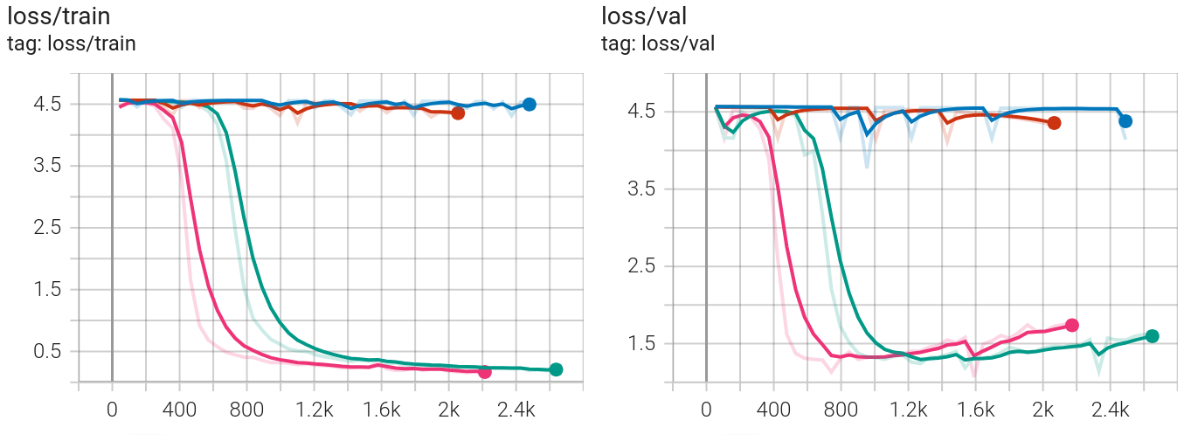
\includegraphics[width=0.8\textwidth]{images/exps2_loss.png}
    \caption{Loss Exps 2}
    \label{fig:exps1_loss}
\end{figure}

Il secondo esperimento evidenzia come, nonostante venga variato il dropout, il fenomeno di overfitting rimanga persistente.

Questo è probabilmente dovuto alla batch size parecchio grande, non consentendo di avere un grado di regolarizzazione sufficiente alto.


\section{Exps 3}

Per ovviare il problema della precedente sperimentazione, si è deciso di ridurre la batch size a \textbf{256}, consentendo di aumentare la regolarizzazione del modello.

Inoltre, un ulteriore tentativo di migliorare il modello si è configurato nella scelta di andare a riutilizzare i migliori pesi man mano che i parametri vengono cambiati. Questo consente di utilizzare un learning rate più basso quando in prossimità del minimo locale.

\begin{figure}[htbp]
    \centering
    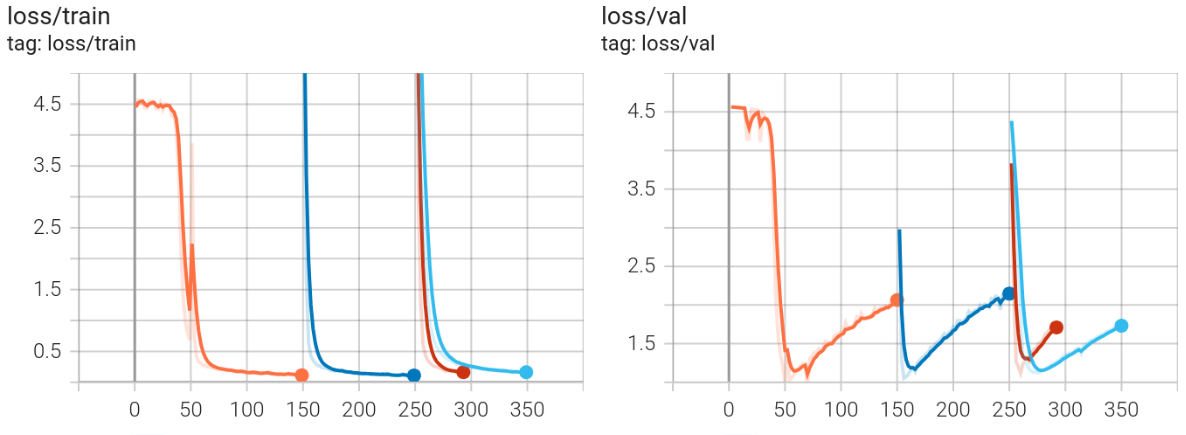
\includegraphics[width=0.8\textwidth]{images/exps3_loss.png}
    \caption{Loss Exps 3}
    \label{fig:exps1_loss}
\end{figure}

I tentativi mostrano uno scarso risultato nel combattere la varianza esibita dalle curve di train e loss.


\section{Exps 4 e 5}



\section{Valutazioni}
\textcolor{red}{INSERIRE intro sul fatto che abbiamo valutato singoli char e frasi}:

\subsection{Singoli caratteri}
La valutazione sui singoli caratteri si articola in due diverse analisi:
\begin{itemize}
    \item Curve Precision-Recall
    \item Matrice di confusione
\end{itemize}

\subsubsection*{Curve Precision-Recall}
Le curve Precision-Recall (PR) consentono di analizzare il bilanciamento tra \emph{precision} e \emph{recall} nelle predizioni del modello, mostrando quanto esso riesca a mantenere alta la precisione man mano che aumenta la quantità di caratteri correttamente riconosciuti. Un indicatore sintetico della qualità complessiva è l'area sotto la curva (AUC-PR), che risulta tanto più elevata quanto migliore è la capacità del modello di conciliare accuratezza e sensibilità nel riconoscimento dei caratteri.

\subsubsection*{Risultati}
In Figura~\ref{fig:pr_curves} sono riportate le curve per un sottoinsieme rappresentativo di classi non confondibili.

\textcolor{red}{INSERIRE quelle nuove (dollaro, Q, T)}:
\begin{figure}[htbp]
    \centering
    \begin{subfigure}[t]{0.32\textwidth}
        \centering
        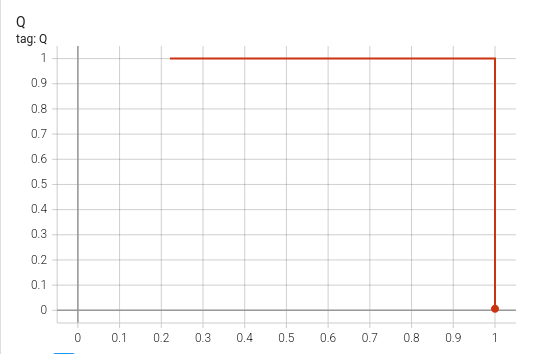
\includegraphics[width=\textwidth]{images/pr_curve1.png}
        \caption{PR-curve \{'\}}
    \end{subfigure}
    \begin{subfigure}[t]{0.32\textwidth}
        \centering
        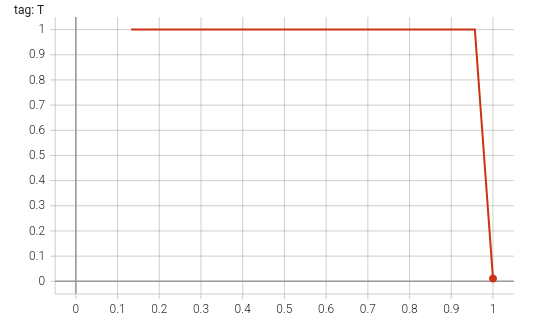
\includegraphics[width=\textwidth]{images/pr_curve2.png}
        \caption{PR-curve \{T\}}
    \end{subfigure}
    \begin{subfigure}[t]{0.32\textwidth}
        \centering
        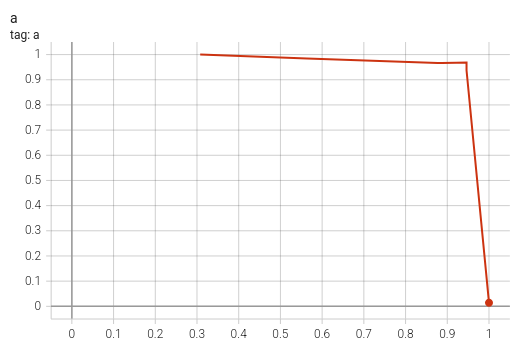
\includegraphics[width=\textwidth]{images/pr_curve3.png}
        \caption{PR-curve \{Y\}}
    \end{subfigure}
    \caption{PR-curves per caratteri non confondibili}
    \label{fig:pr_curves}
\end{figure}

Nel complesso, il modello mostra buone prestazioni, con curve PR ampie e stabili per la maggior parte delle classi.

Tuttavia, alcune classi risultano più problematiche. Come visibile in Figura~\ref{fig:pr-confondibili}.

\textcolor{red}{INSERIRE quelle nuove (c, v, w)}:
\begin{figure}[htbp]
    \centering
    \begin{subfigure}[t]{0.32\textwidth}
        \centering
        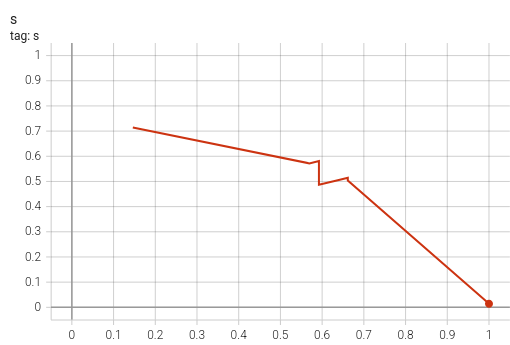
\includegraphics[width=\textwidth]{images/pr_curve_conf1.png}
        \caption{PR-curve \{s\}}
    \end{subfigure}
    \begin{subfigure}[t]{0.32\textwidth}
        \centering
        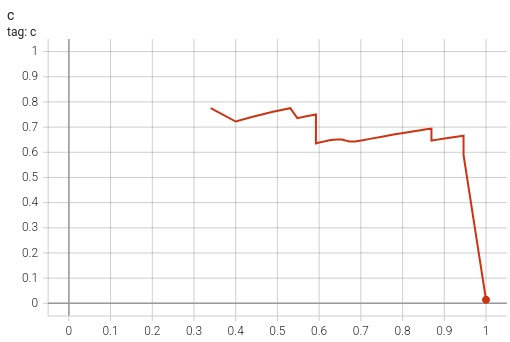
\includegraphics[width=\textwidth]{images/pr_curve_conf2.png}
        \caption{PR-curve \{c\}}
    \end{subfigure}
    \begin{subfigure}[t]{0.32\textwidth}
        \centering
        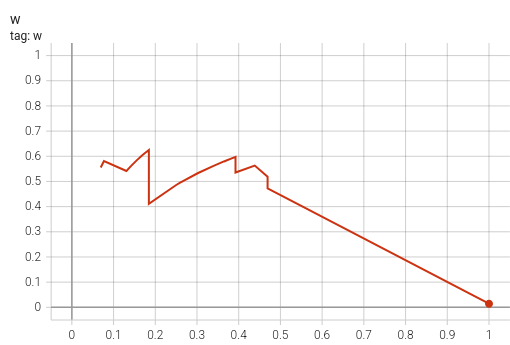
\includegraphics[width=\textwidth]{images/pr_curve_conf3.png}
        \caption{PR-curve \{v\}}
    \end{subfigure}
    \caption{PR-curves per caratteri confondibili}
    \label{fig:pr-confondibili}
\end{figure}

Per valutare l'impatto della distinzione tra maiuscole e minuscole, è stata ripetuta l'analisi ignorando il case. Come mostrato in Figura~\ref{fig:pr-ignore}, l'area sotto la curva migliora sensibilmente, suggerendo che una parte consistente degli errori è dovuta a una difficoltà del modello nel distinguere il case piuttosto che a un'incapacità di riconoscere la forma del carattere.
\textcolor{red}{INSERIRE quelle nuove (c, v, w)}:
\begin{figure}[htbp]
    \centering
    \begin{subfigure}[t]{0.32\textwidth}
        \centering
        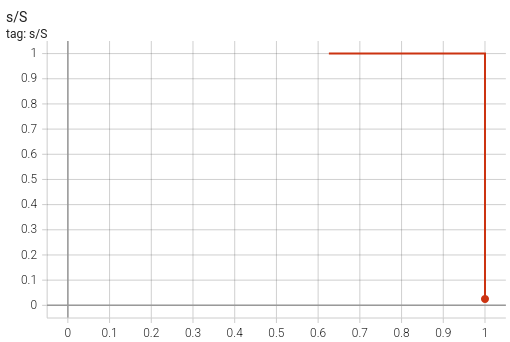
\includegraphics[width=\textwidth]{images/pr_ignore1.png}
        \caption{PR-curve \{s/S\}}
    \end{subfigure}
    \begin{subfigure}[t]{0.32\textwidth}
        \centering
        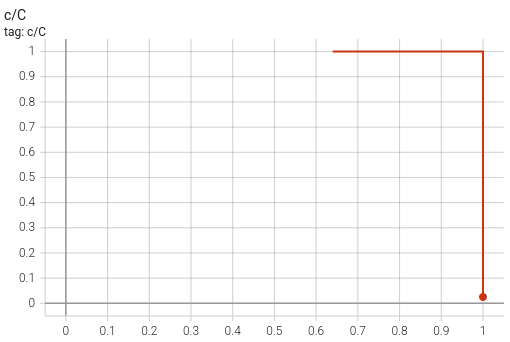
\includegraphics[width=\textwidth]{images/pr_ignore2.png}
        \caption{PR-curve \{c/C\}}
    \end{subfigure}
    \begin{subfigure}[t]{0.32\textwidth}
        \centering
        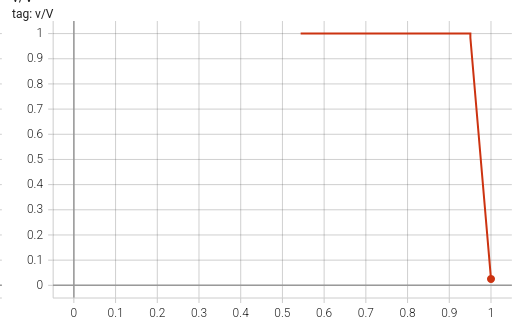
\includegraphics[width=\textwidth]{images/pr_ignore3.png}
        \caption{PR-curve \{v/V\}}
    \end{subfigure}
    \caption{PR-curves ignorando il case}
    \label{fig:pr-ignore}
\end{figure}

\textcolor{red}{INSERIRE caso particolare di [o con lo zero, i con 1]}:
Questi risultati suggeriscono che, pur in presenza di buone prestazioni globali, il modello potrebbe beneficiare delle euristiche di post-processing.


\subsection{Matrice di confusione}
La matrice di confusione aggregata a livello di carattere, mostrata in Figura~\ref{fig:confusion_matrix}, offre una panoramica dettagliata sugli errori di classificazione del modello. Ogni cella \((i, j)\) della matrice rappresenta il numero di volte in cui un carattere \(i\) è stato classificato dal modello come appartenente alla classe \(j\).
\begin{figure}[htbp]
    \centering
    \includegraphics[width=0.65\textwidth]{images/confusion_matrix.png}
    \caption{Matrice di confusione}
    \label{fig:confusion_matrix}
\end{figure}

Si osserva come la diagonale principale della matrice sia in gran parte ben marcata, indicando una prevalenza di classificazioni corrette. Le deviazioni più evidenti dalla diagonale si concentrano invece in corrispondenza di coppie di caratteri visivamente simili, che il modello tende a confondere con maggiore frequenza.

A tal proposito è stata creata un alternativa matrice di confusione che ignora il case, come mostrato in Figura~\ref{fig:confusion_matrix_case_insensitive}. Questa matrice evidenzia che molti errori sono dovuti a questa confusione.
\begin{figure}[htbp]
    \centering
    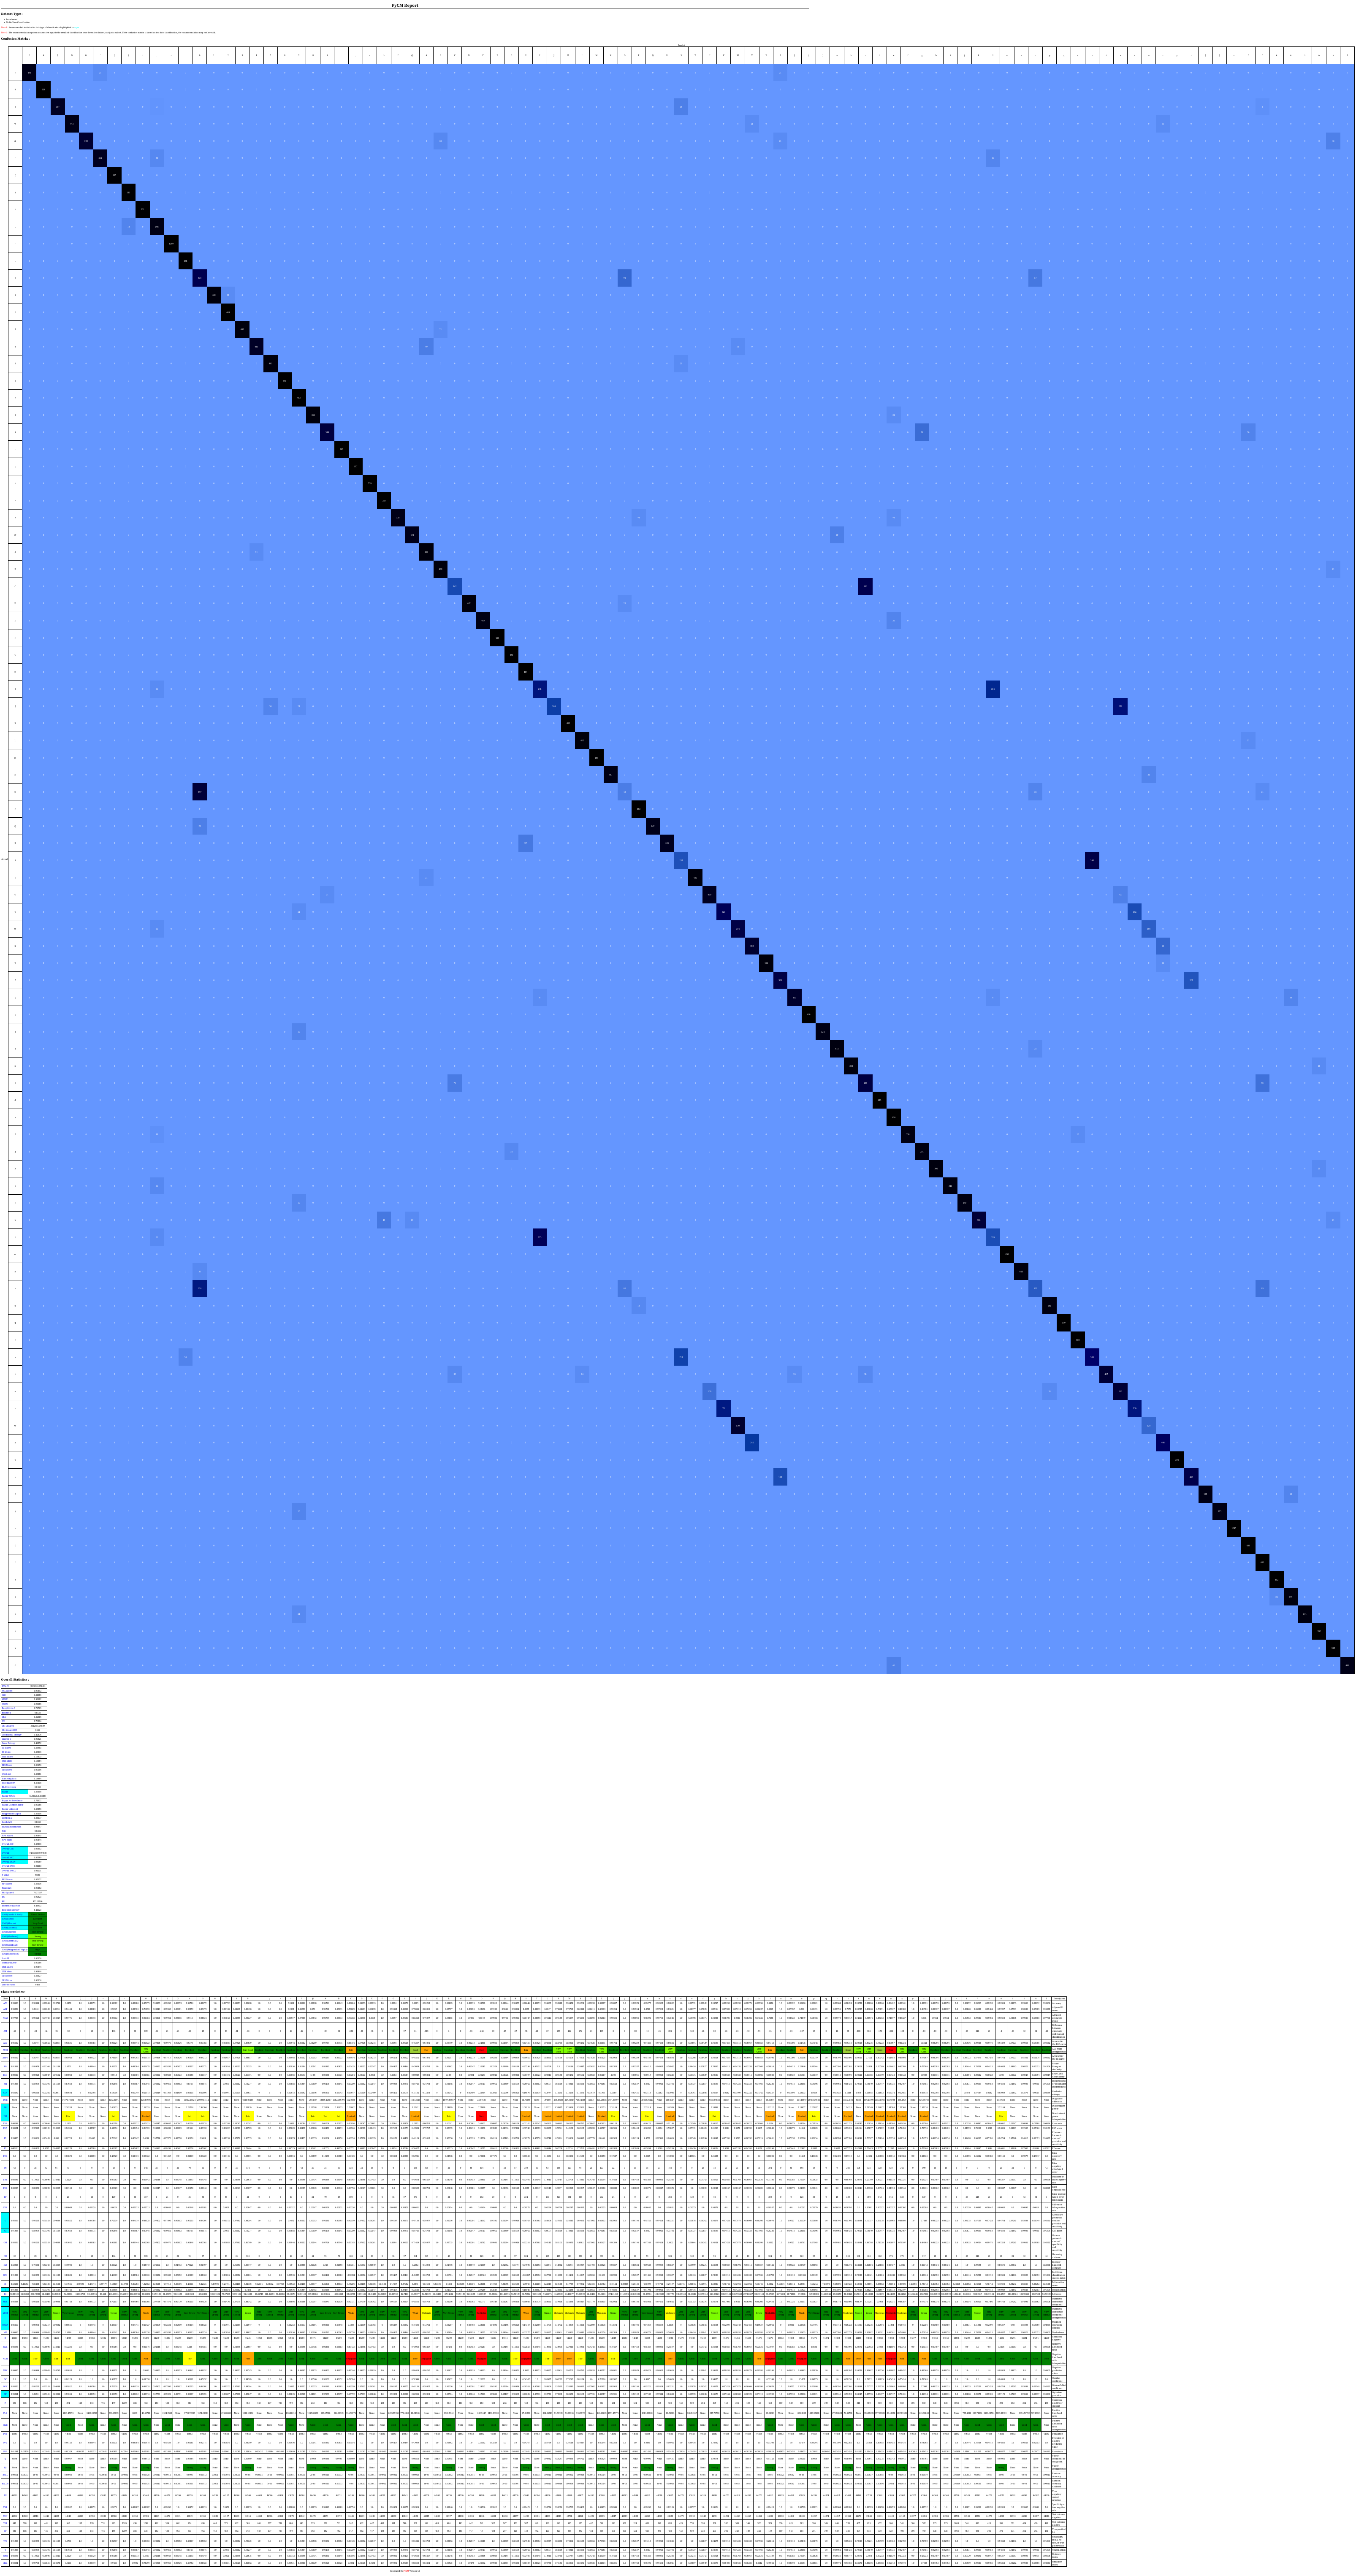
\includegraphics[width=0.65\textwidth]{images/confusion_matrix_case.png}
    \caption{Matrice di confusione ignorando il case}
    \label{fig:confusion_matrix_case_insensitive}
\end{figure}

Questa osservazione conferma la precedente analisi delle PR-curves riguardo i problemi con le classi confondibili.

Nel repository del progetto sono disponibili le matrici di confusione completa sotto forma di report HTML.

\subsection{Valutazione parole}
\label{sec:valutazione-stringhe}

Per l'analisi a livello di parola sono state adottate due metriche principali:
\begin{enumerate}
    \item Distanza di edit (\emph{Levenshtein distance \footnote{V. I. Levenshtein, “Binary codes capable of correcting deletions, insertions and reversals,” \textit{Soviet Physics Doklady}, vol. 10, pp. 707-710, 1966.} });
    \item String Accuracy.
\end{enumerate}

I calcoli sono stati effettuati sui dataset degli screenshot descritti nella \autoref{sec:dataset_screenshots}, che comprendono due tipologie di dati:
\begin{itemize}
    \item sequenze di 10 simboli casuali;
    \item frasi di senso compiuto.
\end{itemize}

\subsection{Distanza di edit}

La distanza di edit tra la parola riconosciuta e la parola ground-truth è stata calcolata per ciascun esempio, normalizzando il valore sulla lunghezza della parola.

Di seguito si riporta una tabella con le statistiche principali (media, mediana e deviazione standard) della distanza di edit normalizzata, calcolate separatamente per i due dataset.

\textcolor{red}{INSERIRE valori reali dopo fix errori}

\begin{table}[htbp]
    \centering
    \begin{tabular}{lccc}
        \toprule
        Dataset & Mean & Median & Std \\
        \midrule
        Sequenze casuali & 0.00 & 0.00 & 0.00 \\
        Frasi di senso compiuto & 0.00 & 0.00 & 0.00 \\
        \bottomrule
    \end{tabular}
    \caption{Statistiche della distanza di edit normalizzata per i due dataset}
    \label{tab:edit_distance_stats}
\end{table}

Dal confronto emerge che il modello si comporta meglio nel riconoscimento delle sequenze casuali rispetto alle frasi di senso compiuto. Ciò può essere dovuto a diversi fattori, tra cui:

\textcolor{red}{DIRE quale può essere il motivo}

\subsection{String Accuracy}
La string accuracy è definita come la percentuale di stringhe riconosciute esattamente nella loro interezza:
\[
    \mathrm{StringAccuracy} = \frac{\text{numero di stringhe perfettamente riconosciute}}{\text{numero totale di immagini}}.
\]

Per una valutazione più dettagliata, sono state considerate tre varianti di string accuracy, che tengono conto di diverse esigenze di confronto:

\begin{itemize}
    \item \textbf{Accuracy case sensitive (CS)}: confronto rigoroso che distingue tra maiuscole e minuscole;
    \item \textbf{Accuracy case insensitive (CI)}: confronto che ignora le differenze tra maiuscole e minuscole, utile per valutare la capacità di distinguere caratteri simili o confondibili;
    \item \textbf{Accuracy case sensitive senza spazi (CSNS)}: confronto che ignora gli spazi ma distingue tra maiuscole e minuscole, utile per valutare la capacità di riconoscimento senza considerare errori di spaziatura.
    \item \textbf{Accuracy case insensitive senza spazi (CINS)}: confronto che ignora sia il case sia gli spazi, utile per gestire eventuali errori di segmentazione o spaziatura

\end{itemize}

La tabella seguente riporta i valori di string accuracy per ciascuna casistica, calcolati separatamente sui due dataset degli screenshot.

\textcolor{red}{INSERIRE valori reali dopo fix errori}

\begin{table}[htbp]
    \centering
    \begin{tabular}{lcccc}
        \toprule
        Dataset                 & CS & CI & CSNS & CINS \\
        \midrule
        Sequenze casuali        & 0.00 & 0.00 & 0.00 & 0.00 \\
        Frasi di senso compiuto & 0.00 & 0.00 & 0.00 & 0.00 \\
        \bottomrule
    \end{tabular}
    \caption{String Accuracy per dataset e casistica di confronto}
    \label{tab:string_accuracy_stats}
\end{table}
